% How to use stdlib_Integrate: the classes a model implements, the time
% schemes that drive it, errors, adding a method. The last section collects
% the design decisions, what later versions would add, and the questions
% still open.
\documentclass[11pt,a4paper]{article}
\usepackage[margin=2.3cm]{geometry}
\usepackage{amsmath,amssymb}
\usepackage{booktabs,array}
\usepackage{graphicx}
\usepackage{xcolor}
\usepackage{listings}
\usepackage[hidelinks]{hyperref}

\newcommand{\dt}{\Delta t}
\newcommand{\code}[1]{\texttt{#1}}
\emergencystretch=3em  % long identifiers: stretch spaces rather than overflow the margin

% Fortran listings: keywords in bold blue, comments in grey italics.
\lstset{
  language=[08]Fortran,
  basicstyle=\ttfamily\small,
  keywordstyle=\bfseries\color{blue!55!black},
  commentstyle=\itshape\color{black!55},
  stringstyle=\color{red!50!black},
  morekeywords={select,type,class,extends,procedure,deferred,abstract,allocatable,%
                intent,inout,error,stop,associate,contains,submodule},
  columns=fullflexible, keepspaces=true,
  frame=single, rulecolor=\color{black!20},
  xleftmargin=1em, xrightmargin=1em, aboveskip=0.8em, belowskip=0.8em,
}

\title{Using \texttt{stdlib\_Integrate}}
\author{}
\date{}

\begin{document}
\maketitle

% ---------------------------------------------------------------------------
\section{Overview}

The library advances the solution of an initial-value problem
$dy/dt = f(t, y)$ in time with explicit Runge--Kutta methods (for the
mathematics, see the textbooks of Butcher~\cite{butcher2016,butcher2021} and
Griffiths and Higham~\cite{gh2010}). It
separates \emph{what} is integrated, which the program provides, from
\emph{how} it is integrated, which the library provides: the program
describes $f$ and the state, the library builds a \emph{time scheme} for a
method and advances the state with it, one step at a time.

How the program describes the problem depends on the shape of its state, and
that is the only decision before writing any code:
\begin{center}
  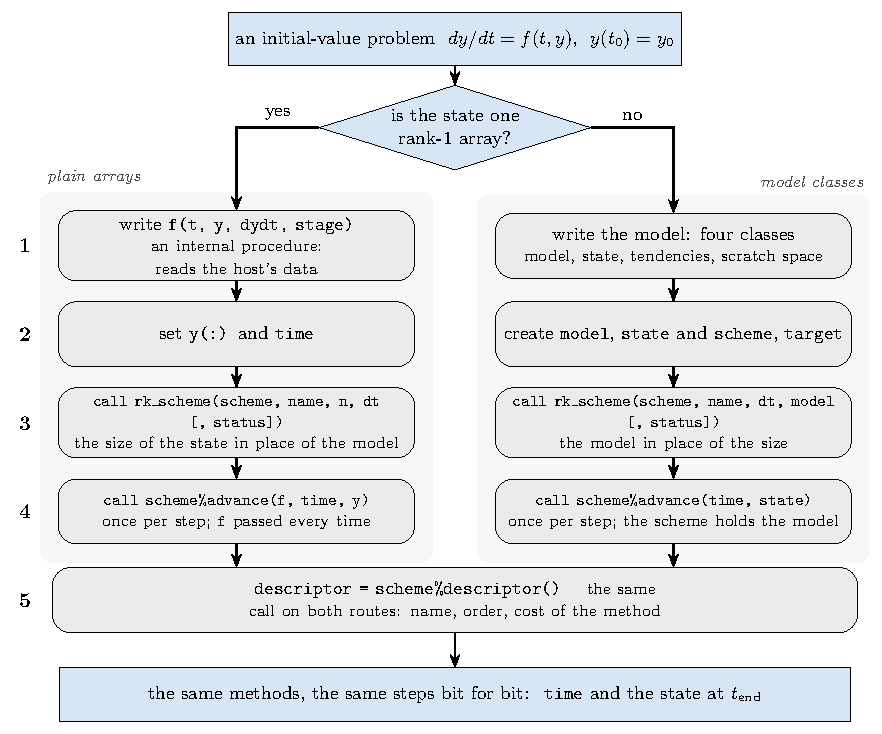
\includegraphics[width=\textwidth]{tikz/pipeline.pdf}
\end{center}
A state that is one rank-1 array needs nothing but a right-hand side
\code{f(t, y, dydt, stage)}. Any other state (several fields, grids, halos,
tiles) is described by four abstract classes the program extends: a model,
its state, its tendencies and a scratch space (section~\ref{sec:model}).
Either way the program goes through the same five steps, and the library runs
the same methods, with the same steps, bit for bit.
Section~\ref{sec:pipeline} walks through both routes, the plain-array one
first as the introductory example; the sections after it explain each part
in full. Everything is re-exported by \code{use stdlib\_Integrate}.

% ---------------------------------------------------------------------------
\section{Using a scheme, step by step}
\label{sec:pipeline}

This section is the road map: what a program does, in order, to integrate a
problem, with each step pointing to the section that explains it in full. It
follows the two branches of the figure in the overview, row by row: plain
arrays when the state is one rank-1 array \code{real(wp) :: y(:)}
(section~\ref{sec:first}), model classes for any other state
(section~\ref{sec:general}). The plain-array route only gives up what a
single array cannot express (several fields, grids, tiles); since both go
through the same five steps, it comes first: it shows the whole pipeline with
nothing in the way.

\subsection{A first program: plain arrays}
\label{sec:first}

Exponential decay, $dy/dt = -\lambda y$ for three values at once, with
classic RK4 at a fixed step, to $t = 1$; the whole program:
\begin{lstlisting}
program decay
    use stdlib_kinds,     only: wp => dp
    use stdlib_Integrate, only: rk_scheme, rk_array_scheme_t, stage_t, &
                                status_t, method_descriptor_t
    implicit none

    real(wp), parameter       :: lambda = 2.0_wp, t_end = 1.0_wp, dt = 0.01_wp
    integer,  parameter       :: n_steps = nint(t_end / dt)
    type(rk_array_scheme_t)   :: scheme
    type(status_t)            :: status
    type(method_descriptor_t) :: descriptor
    real(wp), allocatable     :: y(:)
    real(wp)                  :: time
    integer                   :: it

    y    = [1.0_wp, 2.0_wp, 3.0_wp]                  ! 2. the initial condition
    time = 0.0_wp

    call rk_scheme(scheme, "rk4", size(y), dt, status)   ! 3. the scheme
    if (status%failed) error stop status%message

    do it = 1, n_steps                               ! 4. the time loop
        call scheme%advance(f, time, y, status=status)
        if (status%failed) exit
    end do

    descriptor = scheme%descriptor()                 ! 5. what was run
    print '(a, ": error ", es9.2, ", ", i0, " evaluations")', descriptor%title, &
          maxval(abs(y - [1, 2, 3] * exp(-lambda * time))), &
          n_steps * descriptor%f_evals

contains

    subroutine f(t, y, dydt, stage)                  ! 1. the right-hand side
        real(wp),      intent(in)  :: t, y(:)
        real(wp),      intent(out) :: dydt(:)
        type(stage_t), intent(in)  :: stage
        dydt = -lambda * y                           ! lambda: from the host
    end subroutine f

end program decay
\end{lstlisting}
The five steps, as numbered in the comments:
\begin{enumerate}
  \item \emph{The right-hand side} $f(t, y)$, here an internal procedure: it
    reads \code{lambda} from the program, the closest Fortran has to a
    closure. \code{stage} says which stage of the step the evaluation belongs
    to (section~\ref{sec:stages}); most right-hand sides ignore it.
  \item \emph{The initial condition}: \code{y} and \code{time}, owned by the
    program. The scheme keeps neither.
  \item \emph{The scheme}, built in place by \code{rk\_scheme}: the method by
    name (\code{rk\_method\_names()} lists them), the size of the state, the
    time step. It allocates its buffers here, once. An unknown name fails, in
    \code{status}. The model-class route builds its schemes with the same
    \code{rk\_scheme}, given the model in place of the size
    (section~\ref{sec:general}).
  \item \emph{The time loop}: each \code{advance} moves \code{time} and
    \code{y} one step forward, evaluating \code{f} once per stage. \code{f}
    is passed every time and never stored, so nothing needs to be
    \code{target}. A failure is returned in \code{status}; without it, the
    scheme stops the program with its message.
  \item \emph{What was run}: \code{descriptor()} describes the method (name,
    title, order, evaluations per step; section~\ref{sec:method}).
\end{enumerate}
It prints \code{Classic RK4: error 1.10E-09, 400 evaluations}.

An optional \code{boundaries(t, y, stage)} argument of \code{advance} fills
halos and applies boundary conditions, as a model's \code{apply\_boundaries}
does (section~\ref{sec:arrays}).

\paragraph{When one array is not enough.} The plain-array route stops at a
single rank-1 array: no separate fields, no multi-dimensional arrays without
flattening them by hand, no tiles. The model classes lift all of that: the
library works on the program's own data through the state's procedures. The
same five steps follow, with step 1 becoming a model.

\subsection{The general route: model classes}
\label{sec:general}

\paragraph{1. Write the model.} Four types, each extending an abstract class
of \code{stdlib\_integrate\_model} (section~\ref{sec:model}):
\begin{center}
\renewcommand{\arraystretch}{1.2}
\begin{tabular}{l >{\ttfamily}l p{7.4cm}}
  \toprule
  type & \normalfont extends & must implement \\
  \midrule
  the model      & ODEmodel\_c            & \code{allocate\_state}, \code{allocate\_scratch},
                                            \code{allocate\_tendencies}, \code{compute\_tendencies} \\
  its state      & ODEmodel\_state\_c     & \code{update} ($y \leftarrow y + \text{scale}\cdot k$),
                                            \code{copy} \\
  its tendencies & ODEmodel\_tendencies\_c & nothing: plain data \\
  its scratch    & scratch\_space\_c      & nothing; the base type itself if $f$ needs no
                                            working memory \\
  \bottomrule
\end{tabular}
\end{center}
That is enough for every method. One more procedure is optional:
\code{apply\_boundaries}, when the state has halos or boundary conditions
(section~\ref{sec:model}, ``Halos and boundary conditions''). The smallest
complete model, exponential decay, is \code{examples/decay/decay\_model.f90}
(about 100 lines).

\paragraph{2. Create the model and the state.} Declare them, and the scheme,
\code{target}: the scheme keeps a pointer to the model, and the library passes
the state and its buffers on to procedures that may keep pointers to them
while they run. Set the model's parameters and the
initial condition:
\begin{lstlisting}
use stdlib_Integrate
type(decay_model_t), target               :: model
type(decay_state_t), target               :: state
class(time_scheme_c), allocatable, target :: scheme
type(status_t)                            :: status
real(wp)                                  :: time

model%lambda = 2.0_wp
state%y      = 1.0_wp            ! initial condition y(0)
time         = 0.0_wp
\end{lstlisting}
A program that does not know the state's type at compile time (one driver for
several models) asks the model for it instead, as the scheme does for its own
buffers, and sets the initial condition through \code{select type}:
\begin{lstlisting}
class(ODEmodel_state_c), allocatable, target :: state

call model%allocate_state(state)       ! sized for the model's grid
select type (state)
type is (decay_state_t)
    state%y = 1.0_wp
end select
\end{lstlisting}
A gridded model's allocators size every object for its grid, so the model is
set up (grid read, parameters set) before anything is allocated.

\paragraph{3. Build the scheme.} Always in place, by a subroutine
(section~\ref{sec:schemes}); pick one of
\begin{lstlisting}
! a) a method of the library, by name (the default): rk4's hardcoded step,
!    the generic engine for the others
call rk_scheme(scheme, "rk4", dt, model, status)

! b) any explicit tableau, also one built by hand: the generic engine
call rk_scheme(scheme, rk_tableau("rk3ws"), dt, model, status)

if (status%failed) error stop status%message
\end{lstlisting}
Building allocates every buffer the method needs, once, through the model's
allocators: nothing is allocated inside the time loop. It fails, with a
message in \code{status} and \code{scheme} left unallocated, on an unknown
name, an invalid tableau, or an allocator that allocates nothing. The name can come from a
namelist; \code{rk\_method\_names()} lists the valid ones. The model must
outlive the scheme; the program may change it between steps, and the
scheme sees the change.

\paragraph{4. Run the time loop.} \code{advance(time, state, status)} moves
both \code{time} and \code{state} one step forward
(section~\ref{sec:step}):
\begin{lstlisting}
do it = 1, n_steps
    call scheme%advance(time, state, status)
    if (status%failed) exit                  ! time, state: the last good step
    if (mod(it, n_out) == 0) call write_output(time, state)
end do
\end{lstlisting}
To land exactly on an output time or on the end, shorten the step with
\code{set\_dt}, which changes the time step of every following step:
\code{call scheme\%set\_dt(min(scheme\%get\_dt(), t\_end - time))}. Without
\code{status}, a failed step stops the program with its message
(section~\ref{sec:errors}); with it, the program decides (write a restart,
retry with a smaller \code{dt}, stop).

Two things to know about the state between steps: the program may change it
(a restart, nudging), since every step starts by completing it; and its
halos are stale after \code{advance} returns, so output that reads halos
calls \code{model\%apply\_boundaries} itself first.

\paragraph{5. Ask what was run.} Every scheme describes its method, whatever
its family (section~\ref{sec:method}):
\begin{lstlisting}
type(method_descriptor_t) :: descriptor

descriptor = scheme%descriptor()
print '(a, ": order ", i0, ", ", i0, " evaluations per step")', &
      descriptor%name, descriptor%order, descriptor%f_evals
\end{lstlisting}
The cost of a run is then \code{f\_evals} times the number of steps.

\subsection{Checklist}

The mistakes that do not show up at compile time:
\begin{itemize}
  \item the model is not \code{target}: it usually works, but the scheme's
    pointer to it is not valid Fortran;
  \item the model is a local variable of a routine that returns while the
    scheme lives on: the scheme points to freed memory;
  \item \code{compute\_tendencies} changes its \code{state} argument (it is
    \code{intent(in)}, but a pointer can get around that): the scheme may
    pass the step's own initial state;
  \item the model computes something different from stage to stage without
    meaning to: the method's order no longer holds (section~\ref{sec:stages});
  \item the last step of a fixed-step run overshoots \code{t\_end}:
    \code{n\_steps * dt} must equal the interval, or the last step is
    clipped with \code{set\_dt};
  \item after an interface change, objects compiled against the old one:
    \code{fpm clean --skip} before building.
\end{itemize}

% ---------------------------------------------------------------------------
\section{Writing a model}
\label{sec:model}

A model is four classes, each extending an abstract class of
\code{stdlib\_integrate\_model}:
\begin{center}
\renewcommand{\arraystretch}{1.25}
\begin{tabular}{>{\ttfamily}l p{9.6cm}}
  \toprule
  \normalfont class & role \\
  \midrule
  ODEmodel\_c            & the problem: everything that defines $f$ and does not change
                           in time (grid, parameters, forcing). Allocates the other three
                           objects, applies a state's boundaries (halos, boundary conditions) and
                           evaluates $f$. \\
  ODEmodel\_state\_c     & the degrees of freedom $y$: the fields that evolve. Knows how to
                           copy itself and add scaled tendencies to itself. \\
  ODEmodel\_tendencies\_c & the result $k = f(t, y)$ of one evaluation. May hold fewer
                           fields than the state, if some never change. \\
  scratch\_space\_c      & working memory for evaluating $f$, allocated once and reused
                           (halo copies, intermediate fields). \\
  \bottomrule
\end{tabular}
\end{center}
This section builds the smallest complete model, exponential decay
$dy/dt = -\lambda y$, one class at a time; its full source is
\code{examples/decay/decay\_model.f90}, and \code{fpm run --example decay}
runs it.

\subsection{The model}

The model holds the parameters of $f$ and implements four procedures: three
allocators, called by a scheme when it is built, and the evaluation of $f$,
called once per stage. A fifth, \code{apply\_boundaries}, is optional; it fills a
state's halos and applies its boundary conditions (below).
\begin{lstlisting}
type, extends(ODEmodel_c) :: decay_model_t
    real(wp) :: lambda = 1.0_wp
contains
    procedure :: allocate_state      => decay_allocate_state
    procedure :: allocate_scratch    => decay_allocate_scratch
    procedure :: allocate_tendencies => decay_allocate_tendencies
    procedure :: compute_tendencies  => decay_compute_tendencies
end type
\end{lstlisting}
Each allocator allocates the polymorphic argument with the model's concrete
type, sized for the model (for a gridded model, with the model's grid):
\begin{lstlisting}
subroutine decay_allocate_state(model, state)
    class(decay_model_t),                 intent(in)  :: model
    class(ODEmodel_state_c), allocatable, intent(out) :: state
    allocate(decay_state_t :: state)
end subroutine decay_allocate_state
\end{lstlisting}
The argument is \code{allocatable, intent(out)}, as in the abstract
interface: it arrives deallocated, so the allocator always starts from
nothing, and a scheme being rebuilt never keeps a buffer of an earlier model.
A model that needs no scratch space allocates the base type,
\code{allocate(scratch\_space\_c :: scratch)}.

\paragraph{Evaluating $f$.}
\code{compute\_tendencies(model, status, state, time, scratch, tendencies, stage)}
receives its arguments through the abstract classes, so it first recovers
their concrete types with \code{select type}, then fills \code{tendencies}:
\begin{lstlisting}
select type (state)
type is (decay_state_t)
    select type (tendencies)
    type is (decay_tendencies_t)
        tendencies%dy = -model%lambda * state%y
    end select
end select
\end{lstlisting}
The contract:
\begin{itemize}
  \item \code{state} is \code{intent(in)}: the evaluation must not change it.
    A scheme may pass the step's initial state itself (stage 1, and any stage
    whose stage state equals it), so a change would corrupt the step. The
    state's halos and boundary conditions are already in place: \code{apply\_boundaries}
    has run on it. Intermediate fields (fluxes, divergence, a filtered copy of a
    state field) live in the scratch space, which the evaluation may change
    freely, filling their halos as often as it needs.
  \item \code{time} is the stage time $t_n + c_i\dt$; a model with
    time-dependent forcing must use it rather than a time of its own.
  \item \code{model} is \code{intent(inout)}, so that an evaluation may read
    external data (forcing files) as time advances.
  \item \code{stage} (a \code{stage\_t}) says which stage of the step the
    evaluation belongs to; a model that computes the same $f$ at every stage
    ignores it (below).
  \item On an error, call \code{status\%raise(message)} and return.
\end{itemize}

\paragraph{Stages.}\label{sec:stages} Every engine passes a \code{stage\_t} to
\code{compute\_tendencies} and to \code{apply\_boundaries}:
\begin{center}
\renewcommand{\arraystretch}{1.2}
\begin{tabular}{>{\ttfamily}l p{9.8cm}}
  \toprule
  \normalfont component & meaning \\
  \midrule
  index  & the stage, $1,\dots,s$; stages nothing uses are skipped
           (\code{dp54} evaluates 1 to 6 of 7) \\
  stages & $s$, the method's number of stages \\
  c      & the stage time fraction: the evaluation is at $t_n + c\,\dt$ \\
  dt     & the time step \\
  first  & the first evaluation of the step: on $y_n$ itself, at $t_n$ \\
  last   & the last evaluation of the step: on a stage state, \emph{not} on
           $y_{n+1}$, which no evaluation of the step sees \\
  \bottomrule
\end{tabular}
\end{center}
It lets a model vary what it computes from stage to stage:
\begin{itemize}
  \item \emph{an expensive term computed once per step}: compute it when
    \code{stage\%first}, keep it in the scratch space (the scheme passes the
    same scratch space to every stage of every step) and add the kept value at
    the other stages. That term is then integrated by forward Euler, first
    order in time, whatever the method;
  \item \emph{a stochastic forcing}: draw the increment once per step, when
    \code{stage\%first}, scaled with $\sqrt{\dt}$ (\code{stage\%dt}), and reuse
    it at every stage: all stages of a step must see the same increment.
    Applied to an explicit tableau this gives the simple schemes
    (Euler--Maruyama from forward Euler, the stochastic Heun scheme, which
    converges to the Stratonovich solution, from Heun's method; both run on
    the generic engine from their tableaus); stochastic Runge--Kutta methods
    of higher order need tableaus of their own;
  \item \emph{diagnostics}: of $y_n$ when \code{stage\%first}, reusing what
    \code{compute\_tendencies} computes anyway; the state after the last step
    then needs one more call, or the program computes diagnostics in its own
    loop after \code{advance}.
\end{itemize}
Varying $f$ from stage to stage changes the method: the order of the tableau
no longer applies, and what it becomes is the model's responsibility.

\paragraph{Halos and boundary conditions.} A model whose stencils read halo
points, or whose state has boundary conditions, overrides \code{apply\_boundaries}:
\begin{lstlisting}
subroutine sw_apply_boundaries(model, status, state, time, stage)
    class(sw_model_t),       intent(inout) :: model
    class(status_t),         intent(inout) :: status
    class(ODEmodel_state_c), intent(inout) :: state  ! changed in place
    real(wp),                intent(in)    :: time   ! the stage time
    type(stage_t),           intent(in)    :: stage  ! the stage it is for
    select type (state)
    type is (sw_state_t)
        call fill_halos(state%u)            ! as many fields as needed
        call fill_halos(state%v)
        call fill_halos(state%h)
    end select
end subroutine sw_apply_boundaries
\end{lstlisting}
The scheme calls it on every state before that state is evaluated: once on
\code{state} at the start of each step, and once on each stage state right
after it is built, with that state's time and stage (on \code{state}: the
first stage's). \code{compute\_tendencies} then
always reads a state whose boundaries are applied, without copying it. Starting each step this
way means the program may change \code{state} between steps (a restart,
nudging) or start from one whose halos were never filled. After
\code{advance} returns, the halos of \code{state} are stale until the next
step: output that reads them calls \code{apply\_boundaries} itself.

Filling halos and periodic boundaries only recomputes values from the
interior, so it never changes the solution. A \code{apply\_boundaries} that sets
interior values (prescribed boundary values, clipping, limiters) changes it:
it acts on every stage state and on the state at the start of every step,
the usual convention for stage limiters. The default \code{apply\_boundaries} does
nothing.

\subsection{The state}

The state holds the evolving fields and implements two operations; two
more are optional:
\begin{center}
\renewcommand{\arraystretch}{1.25}
\begin{tabular}{>{\ttfamily}l c p{7.2cm}}
  \toprule
  \normalfont operation & required & meaning \\
  \midrule
  update(status, scale, k)       & yes & $y \leftarrow y + \text{scale}\cdot k$ \\
  copy(status, source)           & yes & $y \leftarrow \text{source}$ (same type; raise an error otherwise) \\
  combine(status, x, c, k)       & no  & $y \leftarrow x + \sum_m c_m k_m$, with $x$ not $y$: builds a stage state \\
  accumulate(status, c, k)       & no  & $y \leftarrow y + \sum_m c_m k_m$: the final update of a step \\
  \bottomrule
\end{tabular}
\end{center}
In \code{combine} and \code{accumulate}, \code{k} is an array of
\code{tendency\_box\_t} (a wrapper, since Fortran has no arrays of
polymorphic objects of different types) and \code{c} holds the coefficients
with $\dt$ already included; zero coefficients are skipped. The defaults are
built from \code{copy} and \code{update}:
\begin{lstlisting}
type, extends(ODEmodel_state_c) :: decay_state_t
    real(wp) :: y = 0.0_wp
contains
    procedure :: update => decay_state_update
    procedure :: copy   => decay_state_copy
end type

subroutine decay_state_update(state, status, scale, tendencies)
    class(decay_state_t),         intent(inout) :: state
    class(status_t),              intent(inout) :: status
    real(wp),                     intent(in)    :: scale
    class(ODEmodel_tendencies_c), intent(in)    :: tendencies
    select type (tendencies)
    type is (decay_tendencies_t)
        state%y = state%y + scale * tendencies%dy
    end select
end subroutine decay_state_update
\end{lstlisting}
\code{copy} is the place for the type check: a \code{class default} branch
raises an error with \code{type\_mismatch(module, procedure, argument, type)}.

\subsection{Tendencies and scratch space}

Both are plain data, with no procedures:
\begin{lstlisting}
type, extends(ODEmodel_tendencies_c) :: decay_tendencies_t
    real(wp) :: dy = 0.0_wp
end type
\end{lstlisting}
A gridded model typically gives its tendencies one field per evolving field
of the state, and its scratch space the intermediate fields of its
right-hand side. In a shallow-water model, for example, the
state is $(u, v, h)$, the tendencies
$(\partial_t u, \partial_t v, \partial_t h)$, and the scratch space holds
gradient, divergence, Laplacian and advection fields; its \code{apply\_boundaries}
fills the halos of $u, v, h$.

% ---------------------------------------------------------------------------
\section{Time schemes}
\label{sec:schemes}

Four words, used with one meaning each in this guide and in the code:
\begin{center}
\renewcommand{\arraystretch}{1.2}
\begin{tabular}{l p{11cm}}
  \toprule
  \emph{method}     & the mathematical object: classic RK4, Dormand--Prince 5(4) \\
  \emph{descriptor} & what describes a method (name, order, error estimate, SSP
                      coefficient, cost): \code{method\_descriptor\_t}, whatever the family
                      (section~\ref{sec:method}) \\
  \emph{definition} & the descriptor plus the coefficients that fully define the
                      method: for an explicit Runge--Kutta method its Butcher tableau,
                      \code{rk\_tableau\_t}, which extends the descriptor \\
  \emph{scheme}     & the method running on a model: bound to the model, with its
                      buffers and time step (\code{time\_scheme\_c}); two schemes can run
                      the same method on two models \\
  \bottomrule
\end{tabular}
\end{center}
A \emph{time scheme} (\code{time\_scheme\_c}) holds a reference to the model,
the time step, and the buffers its method needs (stage states, tendency
registers, scratch space), all allocated once when the scheme is built. Its
only operation is \code{advance}, which moves a state and its time forward by
one step. A program builds a model and a state, builds a scheme, and calls
\code{advance} in its time loop (section~\ref{sec:pipeline}).

\subsection{Choosing a method}

A scheme is built \emph{in place}, by a subroutine, never by a function
returning it: Fortran copies a function's result on assignment, and for a
scheme that copy includes every buffer (section~\ref{sec:design}). Two ways:
\begin{center}
\renewcommand{\arraystretch}{1.25}
\begin{tabular}{>{\ttfamily}l p{8.4cm}}
  \toprule
  \normalfont call & what it builds \\
  \midrule
  rk\_scheme(scheme, name, \dots)    & the method called \code{name}: for \code{"rk4"}, its
                                                   hardcoded step (\code{time\_scheme\_rk4\_t}), unrolled,
                                                   coefficients as constants; for every other method, the
                                                   generic engine on its tableau. The default choice. \\
  rk\_scheme(scheme, tableau, \dots) & the generic engine \code{time\_scheme\_ERK\_t}: a loop
                                                   over any explicit Butcher tableau, including one built
                                                   by hand. On RK4's tableau, the same steps as the
                                                   hardcoded RK4, bit for bit. What a step needs from the
                                                   tableau is computed when the scheme is built. \\
  \bottomrule
\end{tabular}
\end{center}
The full form is \code{rk\_scheme(scheme, name\,|\,tableau, dt, model,
status)}, with \code{scheme} a \code{class(time\_scheme\_c), allocatable}
variable and \code{status} optional.
\code{scheme\%get\_dt()} and \code{scheme\%set\_dt(dt)} read and change the
time step of any scheme.
Method names (\code{rk3ws}, \code{rk4}, \code{dp54}) can come from a
namelist; \code{rk\_method\_names()} lists them.

Building a scheme can fail: an unknown name, an invalid tableau (no stages,
coefficients missing or of the wrong size, not explicit), or a model allocator
that returns without allocating. Like \code{advance}, the constructors return
the failure in the optional \code{status}, with a message, and \code{rk\_scheme}
leaves \code{scheme} unallocated; without \code{status} the failure
stops the program with its message.

The model is kept by reference: it must be declared \code{target} and
outlive the scheme. A program may change the model between steps (an ocean
model reversing its forcing mid-run, say), and the scheme sees the change.

\subsection{Describing a method: the descriptor}
\label{sec:method}

What describes every method, whatever its family, is its descriptor, a
\code{method\_descriptor\_t} (module \code{stdlib\_integrate\_\allowbreak descriptor}).
A family's definition extends it with the coefficients: \code{rk\_tableau\_t}
adds the Butcher tableau ($A$, $b$, $c$, $\hat b$) and the properties only a
Runge--Kutta method has (linear order, FSAL). The tableau's
descriptor is its parent, \code{tab\%method\_descriptor\_t}, and every scheme
returns the descriptor of the method it runs with \code{scheme\%descriptor()},
the hardcoded RK4, the tableau engine and the plain-array schemes alike:
\begin{center}
\renewcommand{\arraystretch}{1.2}
\begin{tabular}{>{\ttfamily}l p{10.4cm}}
  \toprule
  \normalfont component & meaning \\
  \midrule
  name, title, reference & short name (\code{"rk4"}), title, source of the coefficients \\
  order       & order on general (nonlinear) problems \\
  order\_hat  & order of the embedded error estimate; 0 if there is none \\
  explicit    & no equation to solve for the new state (true for every method so far) \\
  ssp\_coef   & SSP coefficient $C$: the step is strong-stability preserving for
                $\dt \le C\,\dt_{\mathrm{FE}}$, with $\dt_{\mathrm{FE}}$ the step at which
                forward Euler is; 0 if not SSP. 0 for the three methods of the library
                (classic RK4 too); 1 for forward Euler, Heun and SSP-RK3 \\
  f\_evals    & tendency evaluations per step: the cost, comparable across methods
                and families \\
  ssp()       & \code{ssp\_coef > 0} \\
  \bottomrule
\end{tabular}
\end{center}
\code{f\_evals} is the method's cost per step: the stages a step evaluates
(\code{dp54} evaluates 6 of its 7). The tableau engine counts the stages it
evaluates, also for a tableau built by hand, whose other components keep
their defaults (0: unknown) unless the program sets them. For the methods of
the library the values are set with the coefficients, and the tests check
the orders against them (section~\ref{sec:adding}).

\subsection{What a step does}
\label{sec:step}

\code{advance(time, state, status)} replaces \code{state} and \code{time}
with their values one step later. For a method with stages $i = 1, \dots, s$
it applies the boundaries of \code{state}, builds each stage state with one \code{combine}
and applies its boundaries, evaluates \code{compute\_tendencies} on it at the stage
time, and finishes with one \code{accumulate} on \code{state}, in place
(the figure leaves out \code{apply\_boundaries}):
\begin{center}
  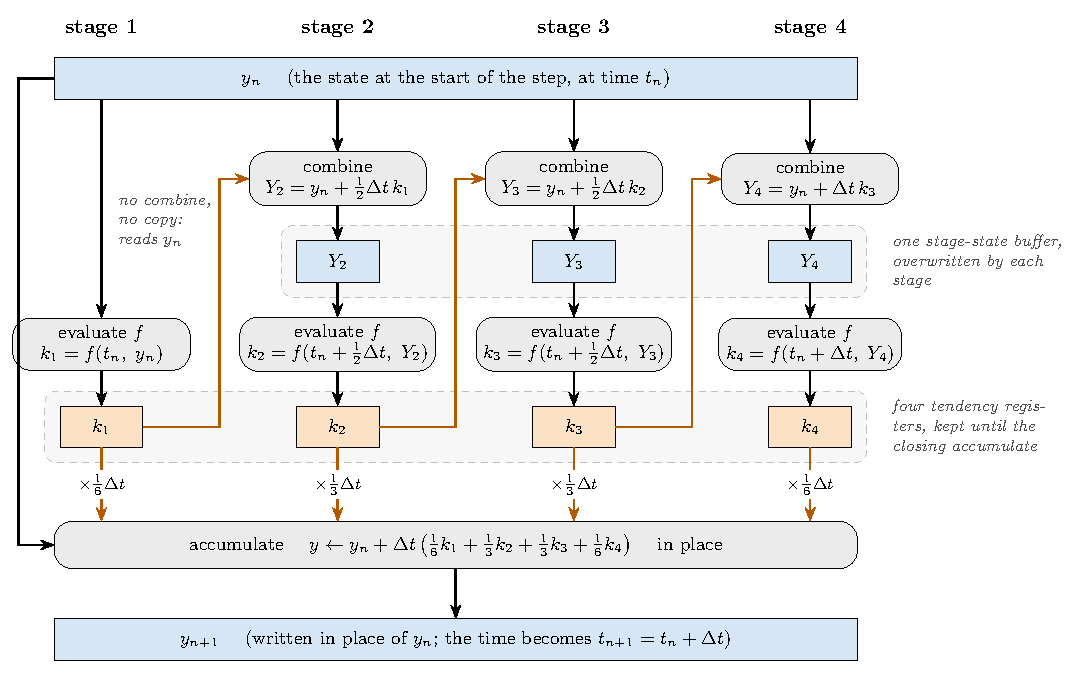
\includegraphics[width=\textwidth]{tikz/rk_step_anatomy.pdf}
\end{center}
The figure draws the classic \code{rk4}. For $y' = f(t, y)$, with $f$ the
model's \code{compute\_tendencies}, its step reads, column by column as in
the figure (each $Y_i$ a \code{combine}, each $k_i$ an evaluation, the last
line the \code{accumulate}):
\begin{alignat*}{2}
  &         &\qquad k_1 &= f(t_n,\ y_n), \\
  Y_2 &= y_n + \tfrac12\dt\, k_1, &\qquad k_2 &= f\bigl(t_n + \tfrac12\dt,\ Y_2\bigr), \\
  Y_3 &= y_n + \tfrac12\dt\, k_2, &\qquad k_3 &= f\bigl(t_n + \tfrac12\dt,\ Y_3\bigr), \\
  Y_4 &= y_n + \dt\, k_3,         &\qquad k_4 &= f\bigl(t_n + \dt,\ Y_4\bigr), \\[3pt]
  y_{n+1} &= y_n + \dt\,\bigl(\tfrac16 k_1 + \tfrac13 k_2 + \tfrac13 k_3 + \tfrac16 k_4\bigr),
  &\qquad t_{n+1} &= t_n + \dt.
\end{alignat*}
The same step drawn as the classical picture, with each object tagged by
the library type that holds it and the call that produces it (exactly for
$y' = -y$, $y_n = 1$, $\dt = 1$):
\begin{center}
  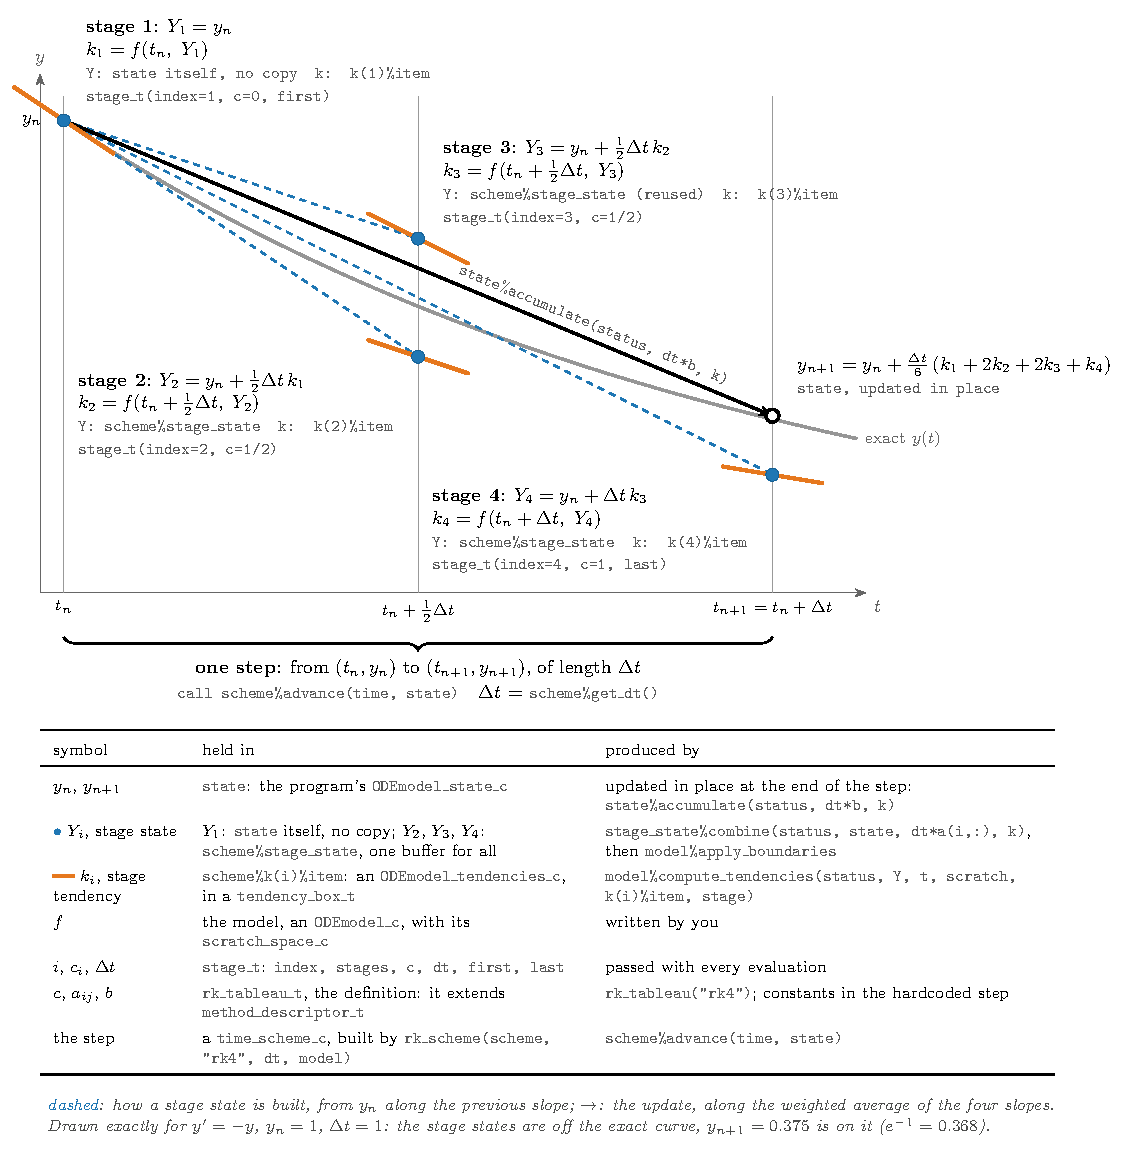
\includegraphics[width=\textwidth]{tikz/rk4_stages.pdf}
\end{center}
A stage whose stage state is the initial state (stage 1, always) evaluates
on \code{state} directly; a stage nothing uses is skipped; and all stage
states share one buffer. The hardcoded RK4 keeps four tendency registers and
one stage state, the fewest its tableau allows (every tendency is read by the
closing update); the generic engine keeps one register per stage (three for
\code{rk3ws}, seven for \code{dp54}, whose seventh stage only an error
estimate would use, and which it skips).

% ---------------------------------------------------------------------------
\section{Plain arrays}
\label{sec:arrays}

A problem whose state is a single rank-1 array needs no model, state or
tendency classes. \code{rk\_array\_scheme\_t} runs the same methods on a
plain array, with a right-hand side \code{f(t, y, dydt, stage)}:
\begin{lstlisting}
use stdlib_Integrate, only: rk_scheme, rk_array_scheme_t, stage_t
type(rk_array_scheme_t) :: scheme
real(wp), allocatable   :: y(:)
real(wp)                :: lambda = 2.0_wp

call rk_scheme(scheme, "rk4", size(y), dt)   ! method name, state size, time step
do it = 1, n_steps
    call scheme%advance(f, time, y)
end do

contains

subroutine f(t, y, dydt, stage)            ! reads lambda from its host
    real(wp),      intent(in)  :: t, y(:)
    real(wp),      intent(out) :: dydt(:)
    type(stage_t), intent(in)  :: stage      ! as for a model; unused here
    dydt = -lambda * y
end subroutine f
\end{lstlisting}
The right-hand side is passed to every \code{advance} and never stored, so
the scheme refers to nothing and needs no \code{target}. It can be an
internal procedure of the caller, as above, which reads the caller's
variables (parameters, a grid) directly: the closest Fortran has to a
closure. An optional \code{boundaries(t, y, stage)} argument fills halos and
applies boundary conditions, called where \code{apply\_boundaries} is called for a
model. \code{stage} is the same \code{stage\_t} a model receives.
The generic \code{rk\_scheme} builds the schemes of both routes, told apart by
the type of \code{scheme} (a \code{type(rk\_array\_scheme\_t)} here). The
arguments follow each route: \code{n, dt} here, \code{dt, model} on the
classes. By name, \code{"rk4"} runs its hardcoded step and every other method
a loop over its tableau; \code{rk\_scheme(scheme, tableau, n, dt, status)} runs
the loop on any explicit tableau, as the generic engine does on the classes.
On a failure the array scheme is left not built (advancing it fails), where
the class route leaves its scheme unallocated.
\code{rk\_scheme} and \code{advance} return their failures (an unknown name, an
invalid tableau, a state of the wrong size, a state that is not contiguous) in
an optional \code{status}, like the class schemes. The state must be a
contiguous array: a strided section would have to be copied in and out at
every step, so it is refused rather than copied behind the caller's back.
\code{get\_dt()} and \code{set\_dt(dt)} read and change the time step, as on the
classes.

\paragraph{Distributed states (MPI).} A state split over processes, each
holding its part flattened into one array with its halo cells, runs on this
route without the classes. Each process builds its own scheme for its local
size, and \code{boundaries} exchanges the halos:
\begin{lstlisting}
call rk_scheme(scheme, "rk4", size(y), dt, status)
do it = 1, n_steps
    call scheme%advance(f, time, y, boundaries=exchange, status=status)
end do

contains

subroutine exchange(t, y, stage)       ! fills the halos of y, whichever array it is
    real(wp),      intent(in)    :: t
    real(wp),      intent(inout) :: y(:)
    type(stage_t), intent(in)    :: stage
    call fill_halos(y, comm)           ! the program's MPI routine; done on return
end subroutine exchange
\end{lstlisting}
(\code{comm} and \code{fill\_halos} are the program's, seen from the host.)
Every process calls \code{boundaries} and \code{f} the same number of times, in
the same order: the stages a method evaluates are fixed. What the program must
respect:
\begin{itemize}
  \item the exchange works on the array it is given: \code{boundaries} is
    called on \code{y} and on the scheme's stage state, two arrays at
    different addresses. Plain sends and receives on the argument (blocking,
    or non-blocking completed before returning) work; persistent requests
    (\code{MPI\_Send\_init}) or RMA windows bound to one buffer do not;
  \item the exchange is finished when \code{boundaries} returns: \code{f}
    receives the array \code{intent(in)}, so MPI may not still be writing
    into it (no overlap of the exchange with the interior computation on
    this route);
  \item \code{f} sets \code{dydt} at the halo cells too (it must define them
    anyway); their values in \code{y} are stale after each step, until the
    next \code{boundaries}.
\end{itemize}

Both routes run the same operations in the same order: the hardcoded RK4 is
the same code on arrays as on classes, and the tableau loop does what the
generic engine does (a stage state is $y_n$, then one term added per nonzero
coefficient; the closing update adds one term per nonzero weight). The two
give the same steps, bit for bit, which the tests check for every method,
built by name and by tableau. Only the implementation differs: each stage is
whole-array expressions and one plain call to \code{f}, with no polymorphism
and no checks per stage. What it gives up: the state is one rank-1 array.

% ---------------------------------------------------------------------------
\section{Errors and reports}
\label{sec:errors}

Every procedure of a model, a state and a scheme takes a \code{status\_t}.
A procedure that fails calls \code{status\%raise(message)}; the scheme stops
the step at the first failure, leaving \code{time} and the state at the last
good step. What happens next depends on the caller:
\begin{itemize}
  \item if it passed \code{status} to \code{advance}, the failure is returned
    there (\code{status\%failed}, \code{status\%message}) and the program
    decides;
  \item otherwise the scheme stops the program with \code{error stop}, and
    the failure's message:
\begin{lstlisting}[language={},frame=none,basicstyle=\ttfamily\footnotesize,breaklines=true,breakindent=2em]
ERROR STOP time_scheme_ERK%advance: time step failed
  type mismatch in decay_model: argument source of decay_state_copy should have type decay_state_t
\end{lstlisting}
\end{itemize}
\code{type\_mismatch(module, procedure, argument, type)} writes the message
for an argument of the wrong type, the usual failure of a \code{select type}
in a model.

% ---------------------------------------------------------------------------
\section{Adding a Runge--Kutta method}
\label{sec:adding}

A program that only needs a method can build its tableau, an
\code{rk\_tableau\_t} with \code{stages}, \code{A}, \code{b} and \code{c}, and
give it to \code{rk\_scheme}: the generic engine runs it on either route, and
nothing in the library changes. Building checks only that the engine can run
it (at least one stage, sizes that match, $A$ strictly lower triangular): a
wrong coefficient is not caught, so a convergence check on a problem with a
known solution is what shows that the coefficients are right.

A method becomes part of the library with a constructor in
\code{src/schemes/rk/stdlib\_integrate\_rk\_tableaus.f90}, as
\code{rk4\_tableau} is written (its coefficients as exact fractions, its
descriptor: name, title, reference, order, linear order, FSAL, SSP coefficient,
evaluations per step), and its name in \code{rk\_tableau} and in
\code{rk\_method\_names}. It then runs on the generic engine, by name, on both
routes, and \code{fpm test} checks it: its order conditions
(\code{test\_RungeKutta\_tableaus}), its convergence
(\code{test\_RungeKutta\_generic}, \code{test\_RungeKutta\_arrays}), its
descriptor (\code{test\_ODEmethod}), the stages it passes
(\code{test\_ODEstage}) and its boundary calls
(\code{test\_ODEmodel\_boundaries}); the last two need its count of calls per
step added to the test.

After changing an interface, run \code{fpm clean --skip} before building:
fpm's incremental build can keep objects compiled against the old interface,
which shows up as a crash at run time. The same applies to programs that use
the library.

\paragraph{Conventions.} The sources follow the style guide of the Fortran
standard library (\code{stdlib}), and new code is written to it:
\begin{itemize}
  \item lowercase keywords, four-space indentation, lines within 132
    characters, \code{intent} on every argument, no \code{dimension}
    attribute, and the name repeated on every \code{end subroutine},
    \code{end function}, \code{end module} and \code{end program};
  \item files end in \code{.f90} (\code{.F90} only for a file that needs the
    preprocessor; none does);
  \item one program unit per file; a submodule lives in
    \code{<parent>\_implementation.f90}, as
    \code{stdlib\_integrate\_rk\_generic\_implementation.f90} does;
  \item a module's tests live in \code{test/test\_<module>.f90}, one program
    each, with any helper module (a test model, say) in a file of its own.
    The test files do not follow the module names yet:
    \code{test\_ODEmodel*} test \code{stdlib\_integrate\_model},
    \code{test\_ODEstage} \code{stdlib\_integrate\_stage},
    \code{test\_ODEmethod} \code{stdlib\_integrate\_descriptor}, and
    \code{test\_RungeKutta\_*} the modules of \code{schemes/rk/}.
\end{itemize}
The test programs:
\begin{center}
\renewcommand{\arraystretch}{1.2}
\begin{tabular}{>{\ttfamily}l p{8.6cm}}
  \toprule
  \normalfont program & what it checks \\
  \midrule
  test\_RungeKutta\_tableaus     & every tableau: explicit, row sums, FSAL, order conditions
                                   up to order 5 \\
  test\_ODEmethod                & the descriptor of every method (\code{method\_descriptor\_t}): the
                                   same from the tableau and from every scheme, by name and by
                                   tableau, on both routes; cost and SSP coefficient; a tableau
                                   built by hand \\
  test\_ODEmodel                 & the default \code{combine} and \code{accumulate},
                                   and \code{copy}'s type check \\
  test\_ODEmodel\_boundaries       & every engine applies the boundaries of every state it evaluates, at its
                                   time, as often as planned; same steps as halos filled on
                                   a scratch copy \\
  test\_ODEstage                 & the \code{stage\_t} every engine passes, for every method, on
                                   both routes: index, stages, $c$, $\dt$, first and last, time
                                   $t_n + c\,\dt$, the first evaluation on $y_n$ \\
  test\_RungeKutta\_construction & every construction failure, which engine a name builds,
                                   rebuilding, the scheme sees later changes to the model \\
  test\_RungeKutta\_arrays       & the plain-array schemes: the same steps and registers as on
                                   classes, bit for bit, by name and by tableau; the hardcoded RK4
                                   against the tableau loop, bit for bit; convergence;
                                   \code{boundaries}; failures \\
  test\_RungeKutta\_methods      & every method by name against the tableau engine, bit for bit;
                                   convergence; registers \\
  test\_RungeKutta\_generic      & convergence of the generic engine, every method \\
  \bottomrule
\end{tabular}
\end{center}

% ---------------------------------------------------------------------------
\section{How the sources are organised}
\label{sec:layout}

Every module is named \code{stdlib\_integrate\_<name>}, in a folder of
\code{src/} by role: \code{model/} for what is integrated (the model contract);
\code{schemes/} for how, shared by every family (\code{scheme},
\code{descriptor}, \code{stage}), with one folder per family
(\code{schemes/rk/}, and one more for each family to come); and
\code{support/} for what both use (\code{status}). The umbrella
\code{stdlib\_Integrate} sits at the top of \code{src/}:
\begin{lstlisting}[language={},frame=none,basicstyle=\ttfamily\footnotesize]
src/
  stdlib_Integrate.f90                     umbrella: use stdlib_Integrate
  support/stdlib_integrate_status.f90      status_t, type_mismatch, fail_step
  model/stdlib_integrate_model.f90         model, state, tendencies, scratch space
  schemes/
    stdlib_integrate_scheme.f90            time_scheme_c, a scheme's buffers
    stdlib_integrate_descriptor.f90        method_descriptor_t
    stdlib_integrate_stage.f90             stage_t
    rk/                                    explicit Runge-Kutta methods
      stdlib_integrate_rk_tableaus.f90     the tableaus, rk_tableau(name), the tableau check
      stdlib_integrate_rk_generic.f90      time_scheme_ERK_t, the generic engine ...
      stdlib_integrate_rk_generic_implementation.f90   ... and its submodule
      stdlib_integrate_rk_steps.f90        time_scheme_rk4_t, rk_scheme on model classes
      stdlib_integrate_rk_arrays.f90       rk_array_scheme_t, rk_scheme on plain arrays
\end{lstlisting}
An arrow means \emph{uses}, leaving out the arrows a longer path implies:
\begin{center}
  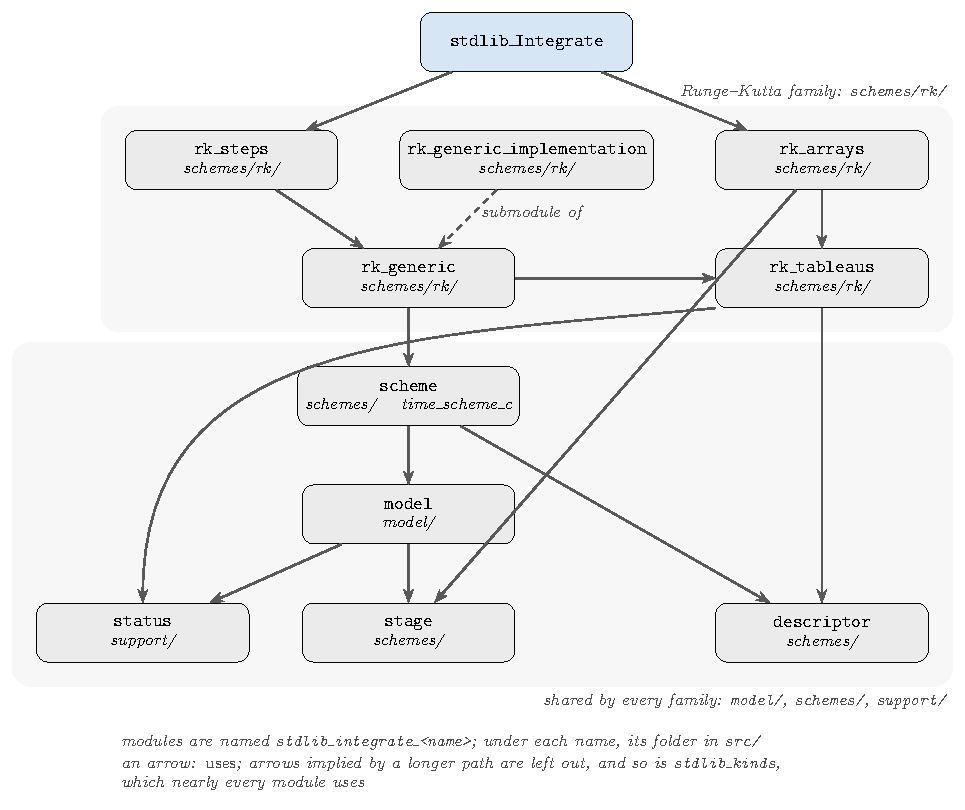
\includegraphics[width=0.9\textwidth]{tikz/dependencies.pdf}
\end{center}
The same graph inverted, at the level of types and procedures: from the
primitives at the top, what is built with each:
\begin{center}
  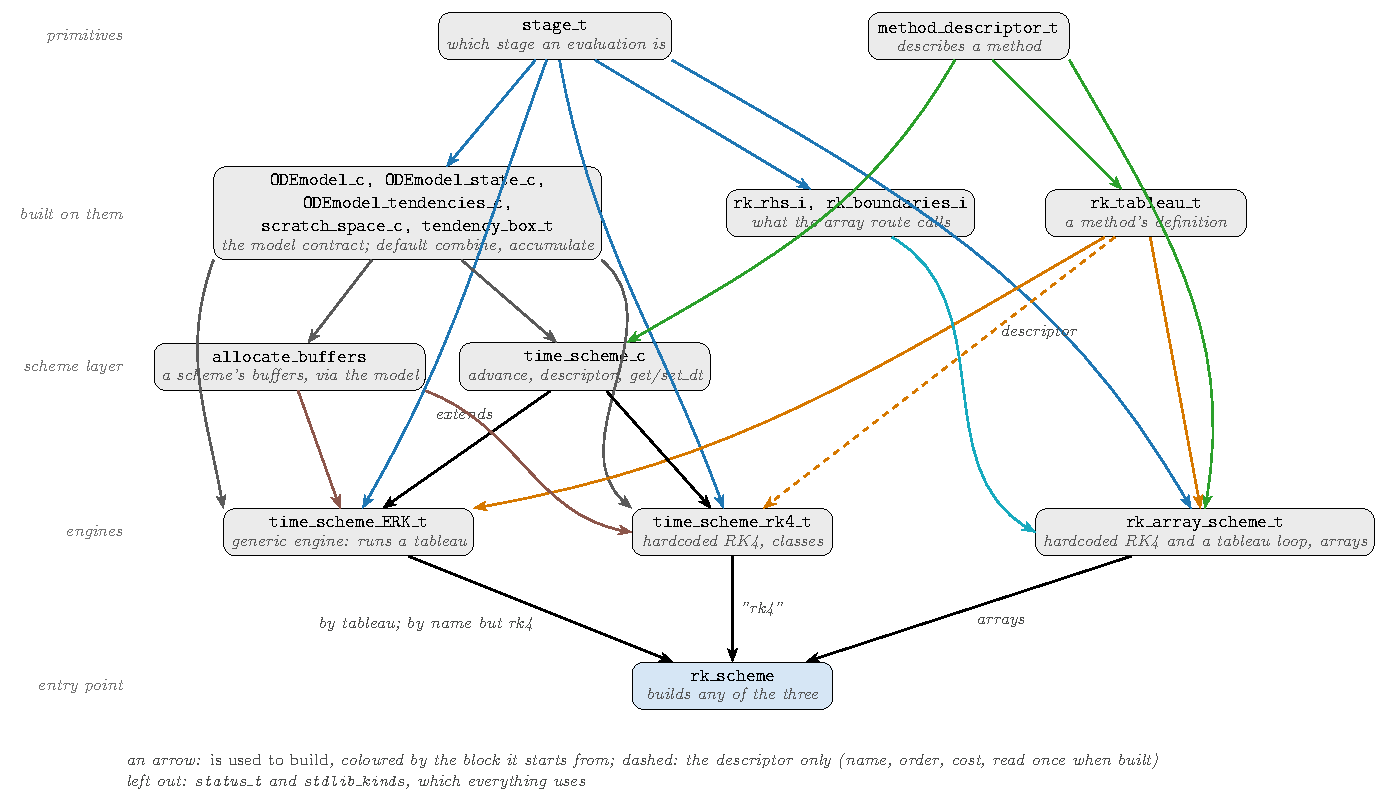
\includegraphics[width=\textwidth]{tikz/building_blocks.pdf}
\end{center}
The array scheme is built from the primitives directly, beside the model
contract rather than on it.

% ---------------------------------------------------------------------------
\section{Design: towards a general-purpose library}
\label{sec:design}

The classes above are designed around one evaluation of $f$ per stage on a
state that is read-only, for models such as ocean, atmosphere and transport
models, whose state is a set of fields on a grid. This section gives the
reasons for the main decisions, what later versions would add, and the open
questions. The library implements one family, explicit Runge--Kutta methods
at fixed steps; how other families (multistep, implicit,
implicit--explicit, partitioned, stochastic) would fit is proposed in
section~\ref{sec:families}.

\subsection{Decided: what a first version contains}
\label{sec:minimal}

\paragraph{The rule.} A first version contains what cannot be added later
without breaking the programs that use it, and leaves out what can. What is
in the signatures of the right-hand side and of the model contract is in it:
the \code{stage} argument, the \code{status} argument, \code{apply\_boundaries}
and \code{boundaries}, and the \code{target} attributes of \code{combine} and
\code{accumulate}, which a one-pass default would need. What can be added as
an optional argument, a procedure with a default or a new method waits for a
later version:
\begin{itemize}
  \item adaptive steps: a step-size controller, the error estimate as an
    operation of the state (with, for a state distributed over processes, a
    reduction that makes it global), counts of accepted and rejected steps,
    and an attempt counter in \code{stage\_t};
  \item one-pass combinations: a state that shows the library its arrays as
    flat views, so that \code{combine} and \code{accumulate} make one pass
    over memory for all terms instead of one \code{update} per term;
  \item low-storage forms, such as Williamson's 2N form, two tendency
    registers whatever the number of stages;
  \item planned steps: a step routine for every method, with its registers
    reused once their tendency is no longer needed, generated and checked
    against the tableau.
\end{itemize}

\paragraph{The methods.} Classic RK4 has a hardcoded step, as the reference
and the most used method; every other method runs on the generic engine, on
both routes, which makes a method a tableau and nothing else. Measured on the
decay model (Apple M4, gfortran 16.1, release build), the engine on RK4's
tableau takes 13\% longer per step than the hardcoded RK4 at $n = 3$ (63
against 55\,ns) and 0.7\% longer at $n = 10^6$, with the same values to the
last bit. It keeps one tendency register per stage (seven for \code{dp54},
where five would do). The tests check the hardcoded RK4 against the engine on
its tableau, bit for bit, on both routes, and every method on arrays against
the classes, bit for bit.

\subsection{Decided: schemes are built in place}

\paragraph{Why.} A function returning a scheme,
\code{scheme = rk\_scheme("rk4", dt, model)}, would return a value: the
assignment copies it into \code{scheme}, deep-copying every allocatable
component, before the result is freed. For a scheme the components are its
buffers, so every buffer would briefly exist twice, and on a large grid peak
memory would nearly double. \code{allocate(scheme, source=...)} copies too,
and \code{move\_alloc} cannot take a function result.

\paragraph{Decision.} Build in place, by one generic subroutine:
\code{rk\_scheme(scheme, name\,|\,tableau, dt, model, status)}, with
\code{scheme} \code{intent(out), allocatable}. Building returns its failures in
\code{status} like \code{advance}, and leaves \code{scheme} unallocated on
failure. The plain-array scheme, a single concrete type that cannot extend
\code{time\_scheme\_c} (its \code{advance} takes the right-hand side and an
array, not a state), is built by the same generic,
\code{rk\_scheme(scheme, name\,|\,tableau, n, dt, status)}; the two are told
apart by the type of \code{scheme}, so both routes build a scheme with the
same call. The tests check every failure path, the unallocated scheme on
failure, which engine a name builds, rebuilding, and that the scheme sees
later changes to the model.

\subsection{Decided: the stdlib style guide}

\paragraph{Decision.} The library follows the contributing guide of the
Fortran standard library, so that it could become part of it (the
conventions of section~\ref{sec:adding} list the rules); the allocators'
argument, for example, is \code{allocatable, intent(out)}.

\paragraph{Still open.} The modules have lowercase names,
\code{stdlib\_integrate\_*}, but for the umbrella \code{stdlib\_Integrate}.
Two steps that change the public interface or the workflow are left for a
decision: lowercase type names (\code{ODEmodel\_c}, \code{time\_scheme\_ERK\_t},
the tableau's \code{A}), which every program using the library would have to
follow; and stdlib's workflow (an experimental namespace first, a
specification page, a CMake build, its test framework).

\subsection{Decided: a hook applies the boundaries of each state}

\paragraph{Why.} \code{compute\_tendencies} receives the state read-only, so
without a hook a model whose stencils read halos would copy each state into
its scratch space to fill the copy's halos: a whole extra pass over every
field on every stage, and a second set of fields in memory.

\paragraph{Decision.} An optional model procedure,
\code{apply\_boundaries(model, status, state, time, stage)}, with the state
\code{intent(inout)}, called by every engine on \code{state} at the start of
each step and on each stage state after its \code{combine}. Halos of
intermediate fields stay in \code{compute\_tendencies}, on the scratch space.
Its counterpart on plain arrays is \code{boundaries}. A halo is a boundary
too, between tiles or processes. The tests check, on every engine, that every
evaluated state had its boundaries applied at its own time starting from
wrong halos, the number of calls (one per step plus one per stage state
built: 3 for \code{rk3ws} to 6 for \code{dp54}), the same steps as a model
filling halos on a scratch copy, and that a failing \code{apply\_boundaries}
fails the step.

\paragraph{Still open.} Whether a third call, after the final
\code{accumulate}, should keep the boundaries of the returned state applied;
the same hook (say \code{finish}) would be the place for end-of-step
diagnostics, which no stage of the step can compute on $y_{n+1}$.

\subsection{Decided: schemes on plain arrays, the same steps}

\paragraph{Why.} A small problem, or one whose state is one array, would pay
for the classes twice: the user writes a model, a state and tendencies, and
each stage pays for dispatch and checks, which dominate on small states.

\paragraph{Decision.} A scheme on plain arrays, with the same methods and
the same operations in the same order as on the classes: the hardcoded RK4
is the same code, and the tableau loop does what the generic engine does. The
right-hand side is an argument of \code{advance}, not stored, so this route
has no pointer at all. Both routes share their calls wherever the arguments
allow: \code{rk\_scheme}, \code{descriptor()}, \code{get\_dt} and
\code{set\_dt}; only \code{advance} differs. Every method gives the same steps
on arrays as on classes, bit for bit, built by name and by tableau; the test
fails if the order of a sum is changed. Ranks above 1 are open.

\subsection{Decided: the stage is passed to the model}

\paragraph{Why.} Some models need to vary what they compute from stage to
stage: an expensive term computed once per step, the increment of a
stochastic forcing drawn once per step and reused at every stage,
diagnostics. The stage's time alone does not identify the stage
(\code{rk4}'s stages 2 and 3 share $c = 1/2$).

\paragraph{Decision.} A small derived type, \code{stage\_t} (module
\code{stdlib\_integrate\_stage}): the stage's index, the method's number of
stages, $c$, $\dt$, and whether the evaluation is the first or the last of
the step. Every engine passes it, \code{intent(in)}, to
\code{compute\_tendencies} and \code{apply\_boundaries} on the class path, and
to the right-hand side and \code{boundaries} on the array path. A derived type
rather than an integer, so that more components can come later (an attempt
counter, with adaptive steps) without changing the interface. What a model
does with it is its own responsibility: a right-hand side that varies between
stages is no longer the method's (section~\ref{sec:stages} lists the uses and
their consequences). \code{test\_ODEstage} checks, for every method and every
engine, the stage passed to each \code{apply\_boundaries} and evaluation,
their order, their times and that the first evaluation sees $y_n$.

\subsection{Decided: a descriptor shared by every family}

\paragraph{Why.} What describes a method (its name, order, error estimate,
whether it is SSP) is not specific to Runge--Kutta methods: kept in the
tableau, a second family would have to repeat it, and a program could not
ask a scheme what it runs without knowing its type.

\paragraph{Decision.} \code{method\_descriptor\_t}
(\code{stdlib\_integrate\_descriptor}, section~\ref{sec:method}) holds what
every family has, and only that; \code{rk\_tableau\_t} extends it. Every scheme
returns it with \code{descriptor()}, its \code{f\_evals} being that scheme's
cost. The names follow one vocabulary: a \emph{method} is the mathematical
object, its \emph{descriptor} what describes it, its \emph{definition} the
descriptor plus its coefficients, a \emph{scheme} the method running on a
model. \code{test\_ODEmethod} checks that the tableau and every scheme give the
same description, and the cost and SSP coefficient of every method.

\subsection{Decided: names and folders by role}

\paragraph{Decision.} One prefix, \code{stdlib\_integrate\_}, as stdlib names
its modules, and folders by role (section~\ref{sec:layout}): \code{model/}
(what is integrated), \code{schemes/} (how, shared by every family, with one
folder per family) and \code{support/} (what both use). Programs that use only
\code{stdlib\_Integrate} never see the module names.

\subsection{Decided: nothing in a step that the step does not need}

\paragraph{Why.} A time integrator is only worth using if it costs no more
than a hand-written loop: every feature free when unused, and no extra pass,
allocation or copy in a step.

\paragraph{Decision.} The generic engine computes which stages are used,
which build a stage state and the last one when it is built, and fills a
buffer of its own with the coefficients, so that a step neither rescans the
tableau nor builds temporaries (\code{dt*A(i,1:i-1)}, which gfortran would
allocate on the heap); the array route's tableau loop does the same, and no
array temporary is left in a step (\code{-Warray-temporaries}). The array
route requires a contiguous state and refuses a strided one, rather than
copying it in and out at every step behind the caller's back, and hands the
steps a contiguous pointer to the state it has checked: handing them the
assumed-shape argument itself costs, measured, about 20\,ns on a 23\,ns step
of \code{rk4} at $n = 3$ and 23\% at $n = 1000$.

\subsection{Proposed: other families of methods}
\label{sec:families}

\paragraph{Problem.} The library covers one family: explicit Runge--Kutta
methods, any tableau with a strictly lower triangular $A$. Other families are
wanted: multistep methods (Adams, BDF), implicit stages (DIRK, SDIRK,
Rosenbrock), implicit--explicit and partitioned methods, stochastic
Runge--Kutta methods, exponential integrators. Each would have a folder of
its own, \code{src/schemes/<family>/}, beside \code{rk/}. The aim is the least infrastructure: share
everything that can be shared, and specialise each family only where it
differs.

\paragraph{The model contract.} It grows by optional procedures, not by new
class hierarchies:
\begin{itemize}
  \item implicit stages: \code{solve(model, status, state, time, gamma\_dt,
    rhs, stage)}, returning the state that satisfies the stage equation
    $Y - \gamma\dt\, f(Y) = r$. The library ships no Newton or Krylov solver:
    the model solves with what it has (a tridiagonal sweep, a multigrid, an
    elliptic solver for a free surface). This is the least infrastructure,
    and for partial differential equations the fastest. A default (Newton
    with a Jacobian-free Krylov method) could come later, as an optional
    helper;
  \item implicit--explicit methods: a second procedure for the implicit part
    of $f$, rather than a flag in \code{stage\_t};
  \item stochastic methods: a procedure for the noise term; the increments
    are drawn once per step by the driver and passed in, rather than frozen
    by the model on the first stage.
\end{itemize}
Each is a type-bound procedure whose default stops with ``method X needs
\code{solve}''; \code{rk\_scheme} checks what a method needs once, when the
scheme is built.

\paragraph{Engines.} Multistep methods (Adams, BDF) carry a history of
tendencies from step to step, so they need an engine of their own, with a
start-up by a Runge--Kutta method; explicit Adams methods, and their
predictor--corrector form, need nothing new from the model, since they only
combine tendencies, and BDF needs the \code{solve} above. Exponential
integrators need the action of matrix functions of the linear part, an
optional model procedure like \code{solve}; they wait for a model that needs
them. Adaptive steps, when they come, are a driver shared by every family: a
step that also returns an error norm, and a controller that accepts or rejects
it and sets the next $\dt$.

\paragraph{Further reading.} For each family, where the three textbooks treat
it (none covers additive, implicit--explicit or low-storage methods; those
need the original papers):
\begin{itemize}
  \item linear multistep methods (Adams, predictor--corrector, BDF):
    \cite[Chs.~4--8]{gh2010}, \cite[Ch.~4]{butcher2016} (starting methods
    Sec.~401, variable step size Sec.~424, predictor--corrector Adams
    methods Sec.~244), \cite[Sec.~6.2]{butcher2021};
  \item implicit and diagonally implicit Runge--Kutta methods, and their
    stability: \cite[Secs.~34--36]{butcher2016} (DIRK: Sec.~361);
  \item Rosenbrock methods, an introduction with one example:
    \cite[Sec.~254]{butcher2016};
  \item symplectic methods and Hamiltonian problems: \cite[Ch.~15]{gh2010},
    \cite[Sec.~39]{butcher2016}, \cite[Ch.~7]{butcher2021};
  \item stochastic differential equations: \cite[Ch.~16]{gh2010};
  \item general linear methods, of which all the above are cases:
    \cite[Ch.~5]{butcher2016}, \cite[Ch.~6]{butcher2021}.
\end{itemize}

\subsection{Still open}
\begin{itemize}
  \item The model is kept by a pointer to a \code{target} argument: it dangles
    if the caller's model is not a \code{target} or goes out of scope, and no
    compiler diagnoses it.
  \item The coefficients $\dt\, a_{ij}$, $\dt\, b_i$ are recomputed at every
    step; they could be computed when the scheme is built, and again when
    \code{set\_dt} changes the step.
  \item The generic engine keeps one tendency register per stage; planning
    which registers a step can reuse (five for \code{dp54} instead of seven)
    is left for a later version.
  \item The state after a failed step, operations on tendencies. Other
    families of methods: section~\ref{sec:families}.
  \item The test files do not follow the module names yet
    (\code{test\_ODEmodel}, \code{test\_RungeKutta\_*}; section~\ref{sec:adding}).
\end{itemize}

% The references of docs/usage.tex, included with % The references of docs/usage.tex, included with % The references of docs/usage.tex, included with \input{bibliography}
% before \end{document}. The three textbooks are the main
% references, cited with a chapter or section for further reading; the papers
% are the original sources of individual methods, for what the books do not
% cover (strong stability preservation, low storage, the coefficients of a
% particular method).
\begin{thebibliography}{9}

\bibitem{butcher2016}
J.~C.~Butcher, \emph{Numerical Methods for Ordinary Differential Equations},
3rd edition, Wiley, 2016. ISBN 978-1-119-12150-3.
Sections are numbered as in the book: Sec.~238 is subsection 8 of
section 23 of chapter 2.

\bibitem{butcher2021}
J.~C.~Butcher, \emph{B-Series: Algebraic Analysis of Numerical Methods},
Springer Series in Computational Mathematics 55, Springer, 2021.
\href{https://doi.org/10.1007/978-3-030-70956-3}{doi:10.1007/978-3-030-70956-3}.

\bibitem{gh2010}
D.~F.~Griffiths and D.~J.~Higham, \emph{Numerical Methods for Ordinary
Differential Equations: Initial Value Problems}, Springer Undergraduate
Mathematics Series, Springer, London, 2010.
\href{https://doi.org/10.1007/978-0-85729-148-6}{doi:10.1007/978-0-85729-148-6}.

\bibitem{shu1988}
C.-W.~Shu and S.~Osher, \emph{J.\ Comput.\ Phys.} 77 (1988) 439.

\bibitem{williamson1980}
J.~H.~Williamson, \emph{J.\ Comput.\ Phys.} 35 (1980) 48.

\bibitem{dormand1980}
J.~R.~Dormand and P.~J.~Prince, \emph{J.\ Comput.\ Appl.\ Math.} 6 (1980) 19.

\bibitem{bogacki1989}
P.~Bogacki and L.~F.~Shampine, \emph{Appl.\ Math.\ Lett.} 2 (1989) 321.

\bibitem{wicker2002}
L.~J.~Wicker and W.~C.~Skamarock, \emph{Mon.\ Wea.\ Rev.} 130 (2002) 2088.

\end{thebibliography}

% before \end{document}. The three textbooks are the main
% references, cited with a chapter or section for further reading; the papers
% are the original sources of individual methods, for what the books do not
% cover (strong stability preservation, low storage, the coefficients of a
% particular method).
\begin{thebibliography}{9}

\bibitem{butcher2016}
J.~C.~Butcher, \emph{Numerical Methods for Ordinary Differential Equations},
3rd edition, Wiley, 2016. ISBN 978-1-119-12150-3.
Sections are numbered as in the book: Sec.~238 is subsection 8 of
section 23 of chapter 2.

\bibitem{butcher2021}
J.~C.~Butcher, \emph{B-Series: Algebraic Analysis of Numerical Methods},
Springer Series in Computational Mathematics 55, Springer, 2021.
\href{https://doi.org/10.1007/978-3-030-70956-3}{doi:10.1007/978-3-030-70956-3}.

\bibitem{gh2010}
D.~F.~Griffiths and D.~J.~Higham, \emph{Numerical Methods for Ordinary
Differential Equations: Initial Value Problems}, Springer Undergraduate
Mathematics Series, Springer, London, 2010.
\href{https://doi.org/10.1007/978-0-85729-148-6}{doi:10.1007/978-0-85729-148-6}.

\bibitem{shu1988}
C.-W.~Shu and S.~Osher, \emph{J.\ Comput.\ Phys.} 77 (1988) 439.

\bibitem{williamson1980}
J.~H.~Williamson, \emph{J.\ Comput.\ Phys.} 35 (1980) 48.

\bibitem{dormand1980}
J.~R.~Dormand and P.~J.~Prince, \emph{J.\ Comput.\ Appl.\ Math.} 6 (1980) 19.

\bibitem{bogacki1989}
P.~Bogacki and L.~F.~Shampine, \emph{Appl.\ Math.\ Lett.} 2 (1989) 321.

\bibitem{wicker2002}
L.~J.~Wicker and W.~C.~Skamarock, \emph{Mon.\ Wea.\ Rev.} 130 (2002) 2088.

\end{thebibliography}

% before \end{document}. The three textbooks are the main
% references, cited with a chapter or section for further reading; the papers
% are the original sources of individual methods, for what the books do not
% cover (strong stability preservation, low storage, the coefficients of a
% particular method).
\begin{thebibliography}{9}

\bibitem{butcher2016}
J.~C.~Butcher, \emph{Numerical Methods for Ordinary Differential Equations},
3rd edition, Wiley, 2016. ISBN 978-1-119-12150-3.
Sections are numbered as in the book: Sec.~238 is subsection 8 of
section 23 of chapter 2.

\bibitem{butcher2021}
J.~C.~Butcher, \emph{B-Series: Algebraic Analysis of Numerical Methods},
Springer Series in Computational Mathematics 55, Springer, 2021.
\href{https://doi.org/10.1007/978-3-030-70956-3}{doi:10.1007/978-3-030-70956-3}.

\bibitem{gh2010}
D.~F.~Griffiths and D.~J.~Higham, \emph{Numerical Methods for Ordinary
Differential Equations: Initial Value Problems}, Springer Undergraduate
Mathematics Series, Springer, London, 2010.
\href{https://doi.org/10.1007/978-0-85729-148-6}{doi:10.1007/978-0-85729-148-6}.

\bibitem{shu1988}
C.-W.~Shu and S.~Osher, \emph{J.\ Comput.\ Phys.} 77 (1988) 439.

\bibitem{williamson1980}
J.~H.~Williamson, \emph{J.\ Comput.\ Phys.} 35 (1980) 48.

\bibitem{dormand1980}
J.~R.~Dormand and P.~J.~Prince, \emph{J.\ Comput.\ Appl.\ Math.} 6 (1980) 19.

\bibitem{bogacki1989}
P.~Bogacki and L.~F.~Shampine, \emph{Appl.\ Math.\ Lett.} 2 (1989) 321.

\bibitem{wicker2002}
L.~J.~Wicker and W.~C.~Skamarock, \emph{Mon.\ Wea.\ Rev.} 130 (2002) 2088.

\end{thebibliography}


\end{document}
